\documentclass[12pt,a4paper]{article}
\usepackage{ctex}
\usepackage{amsmath,amscd,amsbsy,amssymb,latexsym,url,bm,amsthm}
\usepackage{epsfig,graphicx,subfigure}
\usepackage{enumitem,balance}
\usepackage{wrapfig}
\usepackage{mathrsfs,euscript}
\usepackage[usenames]{xcolor}
\usepackage{hyperref}
\usepackage[vlined,ruled,linesnumbered]{algorithm2e}
\usepackage{array}
\hypersetup{colorlinks=true,linkcolor=black}

\newtheorem{theorem}{Theorem}
\newtheorem{lemma}[theorem]{Lemma}
\newtheorem{proposition}[theorem]{Proposition}
\newtheorem{corollary}[theorem]{Corollary}
\newtheorem{exercise}{Exercise}
\newtheorem*{solution}{Solution}
\newtheorem{definition}{Definition}
\theoremstyle{definition}

\renewcommand{\thefootnote}{\fnsymbol{footnote}}

\newcommand{\postscript}[2]
 {\setlength{\epsfxsize}{#2\hsize}
  \centerline{\epsfbox{#1}}}

\renewcommand{\baselinestretch}{1.0}

\setlength{\oddsidemargin}{-0.365in}
\setlength{\evensidemargin}{-0.365in}
\setlength{\topmargin}{-0.3in}
\setlength{\headheight}{0in}
\setlength{\headsep}{0in}
\setlength{\textheight}{10.1in}
\setlength{\textwidth}{7in}
\makeatletter \renewenvironment{proof}[1][Proof] {\par\pushQED{\qed}\normalfont\topsep6\p@\@plus6\p@\relax\trivlist\item[\hskip\labelsep\bfseries#1\@addpunct{.}]\ignorespaces}{\popQED\endtrivlist\@endpefalse} \makeatother
\makeatletter
\renewenvironment{solution}[1][Solution] {\par\pushQED{\qed}\normalfont\topsep6\p@\@plus6\p@\relax\trivlist\item[\hskip\labelsep\bfseries#1\@addpunct{.}]\ignorespaces}{\popQED\endtrivlist\@endpefalse} \makeatother

\begin{document}
\noindent

%========================================================================
\noindent\framebox[\linewidth]{\shortstack[c]{
\Large{\textbf{Lab09-Network Flow}}\vspace{1mm}\\
CS214-Algorithm and Complexity, Xiaofeng Gao \& Lei Wang, Spring 2021.}}
\begin{center}
\footnotesize{\color{red}$*$ If there is any problem, please contact TA Yihao Xie. }

\footnotesize{\color{blue}$*$ Name:Zirui Liu  \quad Student ID:519021910343 \quad Email: L.prime@sjtu.edu.cn}
\end{center}

\begin{enumerate}
    \item  Consider there is a network consists $n$ computers. For some pairs of computers, a wire $i$ exists in the pair, which means these two computers can communicate with each other. When a signal passes through the wires, the noise in the signal will be amplified.If you know the magnification rate of noise $m_{i,j}$ of each wire (which must be greater than 1). Design an algorithm to find the route  for each other computer to send signals to the computer $v$ with the minimum total magnification rate of noise and analyze the time complexity.
	
	\begin{solution}
	This question is almost the same as normal " shortest path problem ". We only have to do such things: \\
	First: We transform all the $m_{i,j}$ to $\log m_{i,j}$ \\
	Second: We apply shortest path algorithm. We can apply Floyd's algorithm since we need to calculate all the computers. The time complexity for Floyd's algorithm is $O\left(n^3\right)$. 
	
	\end{solution}
	
	
	
	
	\item Suppose that we wish to maintain the transitive closure of a directed graph $G=(V,E)$ as we insert edges into $E$. That is, after each edge has been inserted, we want to update the transitive closure of the edges inserted so far. Assume that the graph $G$ has no edges initially and that we represent the transitive closure as a boolean matrix.
	\begin{enumerate}
	    \item Show how to update the transitive closure of a graph $G=(V,E)$ in $O(V^2)$ time when a new edge is added to $G$.
	    \item Give an example of a graph $G$ and an edge $e$ such that $\Omega(V^2)$ time is required to update the transitive closure after the insertion of $e$ into $G$, no matter what algorithm is used.
	    \item Describe an efficient algorithm for updating the transitive closure as edges are inserted into the graph. For any sequence of $m$ insertions, your algorithm should run in total time $\sum_{i=1}^m t_i=O(V^3)$, where $t_i$ is the time to update the transitive closure upon inserting the $i$th edge. Prove that your algorithm attains this time bound.
	\end{enumerate}
	
	\begin{solution}
    (a):\\
    We can update the transitive closure in time $O\left(V^2\right)$ with following prove. We suppose that we add the edge $\left(x_1, x_2\right)$ 
    Then, we will consider every pair of vertices $\left(u, v\right)$. In order to create a path between these two vertices, we need one part of the path which goes from $u$ to $x_1$
    and then other part of the path which goes from $x_2$
    to $v$. This means that we add the edge $\left(u, v\right)$ to the transitive closure if and only if the transitive closure contains the edges $\left(u, x_1\right)$ and $\left(x_2, v\right)$. Since we only had to consider every pair of vertices once, the running time of this update is $O\left(V^2\right)$.

    (b):\\
    Consider inserting the edge $(v_{|V|}, v_1)$ into the graph made of one line $v_1 \to v_2 \to \cdots \to v_{|V|}$.
    Before this edge is inserted, only $|V|(|V| + 1) / 2$ entries in $T$ are $1$. After this edge is inserted, the graph becomes a cycle in which every vertex can reach other vertices, so all $|V|^2$ entries in $T$ are $1$. Hence $|V|^2 - (|V|(|V| + 2) / 2) = \Theta(V^2)$ entries must be changed in $T$, so any algorithms aiming to update the transitive closure will always take $\Omega(V^2)$ time in this case.
    

    (c):\\
    We will have each vertex maintaining a tree of vertices with a path connecting to it. After inserting an edge $\left(u, v\right)$, we will check connecting ancestors of $u$, and add $v$ to their connecting tree, just past $u$. If we  don't insert an edge, we can stop exploring that branch of the ancestor tree. Similarly, we can keep doing this for all the ancestors of $v$. Since we are able to easily check if we ever notice that we have already added an edge, we know that we will only reconsider the same edge at most $n$ times. On the other hand,  since the number of edges is $O\left(n^2\right)$, the total running time is $O\left(n^3\right)$. That is the conclusion.
	
	\end{solution}
	
	
	
	\item An $n\times n$ grid is an undirected graph consisting of n rows and n columns of vertices, as shown in Figure 26.11. We denote the vertex in the $i$th row and the $j$th column by $(i,j)$. All vertices in a grid have exactly four neighbors, except for the boundary vertices, which are the points $(i,j)$ for which $i = 1, i = n, j = 1$, or $j = n$.
    Given $m\leqslant n^2$ starting points $(x_1,y_1), (x_2, y_2), ... , (x_m, y_m)$ in the grid, the escape problem is to determine whether or not there are $m$ vertex-disjoint paths from the starting points to any $m$ different points on the boundary such that every vertex in $V$ is included in at most one of the $m$ paths. For example, the grid in Figure \ref{Fig-EscapeProblem}(a) has an escape, but the grid in \ref{Fig-EscapeProblem}(b) does not.
    \begin{figure}[!htbp]
	\centering
	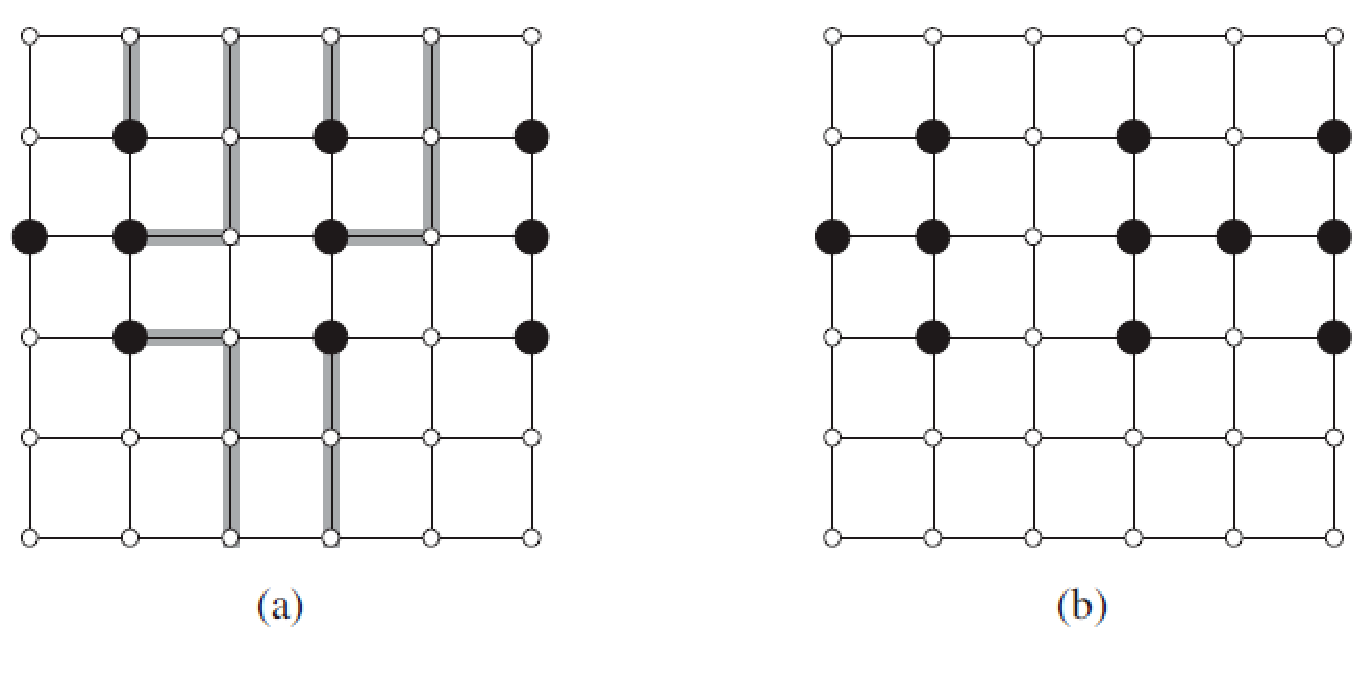
\includegraphics[width=0.5\textwidth]{Fig-EscapeProblem.pdf}
	\caption{Grids for the escape problem. Starting points are black, and other grid vertices are white. (a) A grid with an escape, shown by shaded paths. (b) A grid with no escape.}
	\label{Fig-EscapeProblem}
	\end{figure}
    \begin{enumerate}
        \item Consider a flow network in which vertices, as well as edges, have capacities. That is, the total positive flow entering any given vertex is subject to a capacity constraint. Show that determining the maximum flow in a network with edge and vertex capacities can be reduced to an ordinary maximum-flow problem on a flow network of comparable size. That is, the sizes of the two graph are in the same order of magnitude.
        \item Describe an efficient algorithm to solve the escape problem, and analyze its running time.
    \end{enumerate}
    
    \begin{solution}
	
	(a):\\
	We will now show that a flow network $G = (V, E)$ with vertex capacities can be transformed to an equivalent flow network $G' = (V', E')$ without vertex capacities. \\
	First. We construct $G'$ by dividing each vertex $v$ of $G$ into two vertices $v_1$, $v_2$, joined by an edge of capacity $l(v)$. All incoming edges of $v$ are now incoming edges to $v_1$. All outgoing edges from $v$ are now outgoing edges from $v_2$.

    Secondly, we construct a graph $G' = (V', E')$ with capacity function $c'$ as follows.
    For every $v \in V$, we can create two vertices $v_1$, $v_2$ in $V'$. We add an edge $(v_1, v_2)$ in $E'$ with $c'(v_1, v_2) = l(v)$, and for every edge $(u, v) \in E$, we create an edge $(u_2, v_1)$ in $E'$ with capacity $c'(u_2, v_1) = c(u, v)$. Then we make $s_1$ and $t_2$ to be the new source and destination vertices in $G'$. It is obvious that we have these two equations: $|V'| = 2|V|$ and $|E'| = |E| + |V|$.

    Thirdly, we make $f$ be a flow in $G$ that represents vertex capacities. Then we create a flow function $f'$ in $G'$ as follows. For each edge $(u, v) \in G$, we make $f'(u_2, v_1) = f(u, v)$. For each vertex $u \in V - \{t\}$, we make $f'(u_1, u_2) = \sum_{v \in V} f(u, v)$. After all this, we make $f'(t_1, t_2) = \sum_{v \in V} f(v, t)$.

    Now we can see that there is a one-to-one relationship between flows that represent vertex capacities in $G$ and flows in $G'$. For the capacity constraint, every edge in $G'$ with the form $(u_2, v_1)$ has a corresponding edge in $G$ with a corresponding capacity and flow and thus satisfies the capacity constraint. For edges in $E'$ of the form $(u_1, u_2)$, the capacities reflect the vertex capacities in $G$. As a reason, for $u \in V - \{s, t\}$, we have $f'(u_1, u_2) = \sum_{v \in V} f(u, v) \le l(u) = c'(u_1, u_2)$. We also have $f'(t_1, t_2) = \sum_{v \in V} f(v, t) \le l(t) = c'(t_1, t_2)$. Note this constraint also makes the vertex capacities in $G$.

    Then we will prove flow conservation. By construction, every vertex of the form $u_1$ in $G'$ has exactly one outgoing edge $(u_1, u_2)$, and every incoming edge to $u_1$ corresponds to an incoming edge of $u \in G$. Thus, for all vertices $u \in V - \{s, t\}$, we have

    $$ \begin{aligned} \text{incoming flow to $u_1$} & = \sum_{v \in V'} f'(v, u_1) \\ & = \sum_{v \in V} f(v, u) \\ & = \sum_{v \in V} f(u, v) \qquad \\ & = f'(u_1, u_2) \\ & = \text{outgoing flow from $u_1$}. \end{aligned} $$

    For $t_1$, we can have that

    $$ \begin{aligned} \text{incoming flow} & = \sum_{v \in V'} f'(v, t_1) \\ & = \sum_{v \in V} f(v, u) \\ & = f'(t_1, t_2) \\ & = \text{outgoing flow}. \end{aligned} $$

    Vertices of the form $u_2$ have exactly one incoming edge $(u_1, u_2)$, and every outgoing edge of $u_2$ equals to an outgoing edge of $u \in G$. Thus, for $u_2 \ne t_2$,

    $$ \begin{aligned} \text{incoming flow} & = f'(u_1, u_2) \\ & = \sum_{v \in V} f(u, v) \\ & = \sum_{v \in V'} f'(u_2, v) \\ & = \text{outgoing flow}. \end{aligned} $$

    From this, we can finally prove that $|f'| = |f|$:

    $$ \begin{aligned} |f'| & = \sum_{v \in V'} f'(s_1, v) \\ & = f'(s_1, s_2) \qquad  \\ & = \sum_{v \in V} f(s, v) \\ & = |f|. \end{aligned} $$
	
	(b):\\
	We can construct a vertex of constrained flow network by letting our flow network have a vertex, each with a unit capacity(can be equal or not), for each point on the grid lines, having a two way edge with unit capacity for each pair of vertices that are adjacent on  the grid. Then, we put a unit capacity edge going from $s$ to each of the distinguished vertices, and a unit capacity edge going from each vertex on the sides of the grid to $t$. Then we know that a solution to this problem will be the same as a solution to the escape problem because all the augmented paths will be a unit flow, since every edge has a unit capacity. This means that the flows through the grid will be the paths we choose. This fact gives us the escaping paths if the total flow is equal to $m$, since we know we will not have greater than $m$ by looking at the cut which has $s$ by itself. On the other hand, if the max flow is less than $m$, we know that the escape problem is not solvable, because otherwise we could construct a flow with value $m$ from the list of disjoint paths that the escaping path goes along.
	
	
	\end{solution}
    
    
    
\end{enumerate}

\textbf{Remark:} Please include your .pdf, .tex files for uploading with standard file names.
\newpage


%========================================================================
\end{document}